%% For double-blind review submission, w/o CCS and ACM Reference (max submission space)
\documentclass[sigplan,review,anonymous=false]{acmart}\settopmatter{printfolios=true,printccs=false,printacmref=false}
%% For double-blind review submission, w/ CCS and ACM Reference
%\documentclass[sigplan,review,anonymous]{acmart}\settopmatter{printfolios=true}
%% For single-blind review submission, w/o CCS and ACM Reference (max submission space)
%\documentclass[sigplan,review]{acmart}\settopmatter{printfolios=true,printccs=false,printacmref=false}
%% For single-blind review submission, w/ CCS and ACM Reference
%\documentclass[sigplan,review]{acmart}\settopmatter{printfolios=true}
%% For final camera-ready submission, w/ required CCS and ACM Reference
%\documentclass[sigplan]{acmart}\settopmatter{}


%% Conference information
%% Supplied to authors by publisher for camera-ready submission;
%% use defaults for review submission.

\acmConference[]{}
\acmYear{}
\acmISBN{} % \acmISBN{978-x-xxxx-xxxx-x/YY/MM}
\acmDOI{} % \acmDOI{10.1145/nnnnnnn.nnnnnnn}
\startPage{1}

%% Copyright information
%% Supplied to authors (based on authors' rights management selection;
%% see authors.acm.org) by publisher for camera-ready submission;
%% use 'none' for review submission.
\setcopyright{none}
%\setcopyright{acmcopyright}
%\setcopyright{acmlicensed}
%\setcopyright{rightsretained}
\copyrightyear{}           %% If different from \acmYear

%% Bibliography style
\bibliographystyle{ACM-Reference-Format}
%% Citation style
%\citestyle{acmauthoryear}  %% For author/year citations
%\citestyle{acmnumeric}     %% For numeric citations
%\setcitestyle{nosort}      %% With 'acmnumeric', to disable automatic
                            %% sorting of references within a single citation;
                            %% e.g., \cite{Smith99,Carpenter05,Baker12}
                            %% rendered as [14,5,2] rather than [2,5,14].
%\setcitesyle{nocompress}   %% With 'acmnumeric', to disable automatic
                            %% compression of sequential references within a
                            %% single citation;
                            %% e.g., \cite{Baker12,Baker14,Baker16}
                            %% rendered as [2,3,4] rather than [2-4].


%%%%%%%%%%%%%%%%%%%%%%%%%%%%%%%%%%%%%%%%%%%%%%%%%%%%%%%%%%%%%%%%%%%%%%
%% Note: Authors migrating a paper from traditional SIGPLAN
%% proceedings format to PACMPL format must update the
%% '\documentclass' and topmatter commands above; see
%% 'acmart-pacmpl-template.tex'.
%%%%%%%%%%%%%%%%%%%%%%%%%%%%%%%%%%%%%%%%%%%%%%%%%%%%%%%%%%%%%%%%%%%%%%


%% Some recommended packages.
\usepackage{booktabs}   %% For formal tables:
                        %% http://ctan.org/pkg/booktabs
\usepackage{subcaption} %% For complex figures with subfigures/subcaptions
                        %% http://ctan.org/pkg/subcaption
\usepackage{lmodern}
\usepackage{graphicx}
\graphicspath{ {images/} }

\begin{document}

%% Title information
\title[Short Title]{Exploring Floating-Point Trade-Offs in Machine Learning}         %% [Short Title] is optional;
                                        %% when present, will be used in
                                        %% header instead of Full Title.
\titlenote{Both Vanilla and Average variants of the Perceptron algorithm}             %% \titlenote is optional;
                                        %% can be repeated if necessary;
                                        %% contents suppressed with 'anonymous'
%\subtitle{Subtitle}                     %% \subtitle is optional
%\subtitlenote{with sudddddbtitle note}       %% \subtitlenote is optional;
                                        %% can be repeated if necessary;
                                        %% contents suppressed with 'anonymous'


%% Author information
%% Contents and number of authors suppressed with 'anonymous'.
%% Each author should be introduced by \author, followed by
%% \authornote (optional), \orcid (optional), \affiliation, and
%% \email.
%% An author may have multiple affiliations and/or emails; repeat the
%% appropriate command.
%% Many elements are not rendered, but should be provided for metadata
%% extraction tools.

%% Author with single affiliation.
\author{First1 Last1}
\authornote{with author1 note}          %% \authornote is optional;
                                        %% can be repeated if necessary
\orcid{nnnn-nnnn-nnnn-nnnn}             %% \orcid is optional
\affiliation{
  %\position{Position1}
  %\department{Department1}              %% \department is recommended
  \institution{Institution1}            %% \institution is required
  %\streetaddress{Street1 Address1}
  %\city{City1}
  %\state{State1}
  %\postcode{Post-Code1}
  %\country{Country1}                    %% \country is recommended
}
\email{first1.last1@inst1.edu}          %% \email is recommended

%% Author with two affiliations and emails.
\author{First2 Last2}
\authornote{with author2 note}          %% \authornote is optional;
                                        %% can be repeated if necessary
\orcid{nnnn-nnnn-nnnn-nnnn}             %% \orcid is optional
\affiliation{
  %\position{Position2a}
  %\department{Department2a}             %% \department is recommended
  \institution{Institution2a}           %% \institution is required
  %\streetaddress{Street2a Address2a}
  %\city{City2a}
  %\state{State2a}
  %\postcode{Post-Code2a}
  %\country{Country2a}                   %% \country is recommended
}
\email{first2.last2@inst2a.com}         %% \email is recommended


%% Abstract
%% Note: \begin{abstract}...\end{abstract} environment must come
%% before \maketitle command
\begin{abstract}
	
Both Perceptron and SVM algorithms are two well known linear predictors. The weight vector has the goal of model it self to the training set, for later performing on unknown data.
The training and testing of these two algorithms is usually performed using IEEE 754 double precision. 
The main goal of this work is to analyze what is the impact of FP precision adopted for reading the dataset, compute the training and at the end testing it, on the final accuracy of the predictor. 
Our analysis spans the really poor values of the floating point range, and compare these results with respect to well known IEEE defined standards: single and double precision.
\end{abstract}


%% 2012 ACM Computing Classification System (CSS) concepts
%% Generate at 'http://dl.acm.org/ccs/ccs.cfm'.
\begin{CCSXML}
<ccs2012>
<concept>
<concept_id>10011007.10011006.10011008</concept_id>
<concept_desc>Software and its engineering~General programming languages</concept_desc>
<concept_significance>500</concept_significance>
</concept>
<concept>
<concept_id>10003456.10003457.10003521.10003525</concept_id>
<concept_desc>Social and professional topics~History of programming languages</concept_desc>
<concept_significance>300</concept_significance>
</concept>
</ccs2012>
\end{CCSXML}

\ccsdesc[500]{Software and its engineering~General programming languages}
\ccsdesc[300]{Social and professional topics~History of programming languages}
%% End of generated code


%% Keywords
%% comma separated list
\keywords{keyword1, keyword2, keyword3}  %% \keywords are mandatory in final camera-ready submission


%% \maketitle
%% Note: \maketitle command must come after title commands, author
%% commands, abstract environment, Computing Classification System
%% environment and commands, and keywords command.
\maketitle

\section{Introduction}
A lot of different works studied the impact of low precision computations on machine learning predictors. 
Gupta et al\cite{gupta} focuses the analysis on fixed-point arithmetic, with a particular emphasis on rounding mode of fixed-point operations because considered one of the main actor in the success of low cost arithmetic. The authors prove that deep neural network can be trained using fixed-point arithmetic at low precision. They show how using fixed point with 16 bit precision produces same results of single floating point (32 bit precision). 

Zhou et al. in \cite{dorefa} proposes innovative  methods to train convolutional neural networks that
have low bit-width weights, activations step and parameter gradients. In particular they show how using 1 bit weight, 1 bit activation and 2 bit gradient achieve a value of 93\% of accuracy compare to 97\% obtained with 32 bit single precision. 
At the same time using 1A,1G and 8G bit configuration reaches exactly the same accuracy than the 32 bits counter part.

Hubara et al.\cite{Hubara} introduces a method to train Quantized-Neural-Networks (QNNs) with low precision weights and activations and they reach the same results as single precision 32 bit. 
In particular, using 4 bits for weights and activation, the degradation of the accuracy is 5.5\% compared to 32 bit single precision. Moreover, they report an approximate 5.6\% drop in performance (top-1 accuracy) compared to 32-bit floating
point representation, using only 1-bit for weights and 2-bit for activation step.

At the same time we are aware of many floating point analyzer that could be applied to a black box algorithm to detect the minimal configuration of each floating point instructions in the program, with the goal of minimizing the final error \cite{reducelam}\cite{mixpreclam}\cite{precimonious}\cite{blame}. 

Program analysis applied to floating point instructions usually maintains few 'ghosts' executions that replicate the behavior of the program under different floating point precisions.\cite{blame}\cite{precimonious}. The result of the tuning of the instructions is injected into the binary code of the program and the candidate result may be evaluated again.\cite{mixpreclam}\cite{reducelam}.

%In particular, the aim of these tools is to produce the minimal configuration of FP instructions such that the output keeps same quality. 
%These techniques involve both static and dynamic approaches: usually the first is used to detect FP instructions in the program, while the second one produces improvement on the configuration of the solution, also due to 'ghost' executions that verify the current configuration.

Our analysis admire and look forward these analyzers, but our goal move away from the detection of the minimal FP configuration of Perceptron and SVM such that a given value of accuracy is reached. What we do indeed is to study what are the behaviors of the accuracy of these predictors for really poor FP precision computations. 

In particular, we want to compare the accuracy of the predictors ($\frac{Correct.Prediction}{Tot.Samples}$) in case of really poor floating point precision (from 2 to 10 bits for mantissa representation) and compare them to well know (expensive) single and double IEEE 754 double precision. 

Most of the times FP analyzer arbitrarily fixed the range to span of all the possible floating point precision until double (eg. all double configuration represent the worst case in terms of FP efficiency and energy consumption). 

Our work concentrates the results on tuning the precision of mantissa, because it may show gradual improvement on the final accuracy, that is directly proportional to the number of bits assigned to the representation. 
On the other hand, the exponent does not show such behavior. When a given amount of bits n does not produce an overflow (or underflow) in the computation, testing the exponent range using $m>n$ bits dedicated to dynamic range has no impact on the accuracy of the algorithm. 

\section{Background}
One way real numbers can be discretized in the machine is using floating point representation. The format adopted for the representation is the following: sign of the number, significant (mantissa) and exponent. The  value is then represented with $(-1)^{sign} \cdot significand \cdot 2^{exponent}$. 
The floating point representation is part of the IEEE 754 standard that, among the others, includes two well known representations: single precision (1bit sign, 23bits mantissa, 8bits exponent) and double precision (1bit sign, 52bits mantissa, 11bits exponent). 
These are the most common representations used for FP computations. It has been showed in \cite{softfloat} that most of the time the way the total number of bits is divided in mantissa and exponent (1 bit sign always exists) it is not the best possible and better results can be obtained by reassigning the number of bits in different ways\cite{softfloat}.

%\section{Perceptron and SVM}
\subsection{Perceptron and SVM}
The Perceptron algorithm is a supervised learning algorithm invented by Frank Rosenblatt in 1957\cite{perceptron}. The goal of the predictor is to built a  linear decision boundary on the training set and to classify future samples based on such classifier. To reach such goal, the Perceptron updates the coordinates of the hyperplane such that the linear bounds will come closer to the misclassified sample. 
The Perceptron is a mistake driven algorithm: once a sample is misclassified the predictor is corrected (it does not mean that the sample now is correctly classified).
Particularly interesting in terms of FP analysis is one of the variant of the vanilla Perceptron: the Average Perceptron. 
The Average Perceptron differs from the vanilla version because it maintains an average vector weighted on the misclassification occurred until the current iteration. 
Our interests about FP analysis comes from the necessity of more FP computational range to compute the average of the 'accumulator' boundary, on the other hand usually the average version performs better than the vanilla one.

Also SVM algortihm produces a linear classifier but it differs from Perceptron in the the way the hyperplane is obtained. Indeed, SVM requires not only that the predictor learns from the training set, but it also aims for a safe margin between the linear separator and the closest points. For this reason it is learning by maximizing margin. It exists two versions of the classifier: (i) hard SVM means that no point are allowed to live between the linear separator and the margin and (ii) soft SVM allows that kind of points to exists and tries to minimize these points. The goal here is to maximize the 'safe' margin together with the correct classification of the training set.

\section{Methodology}
\subsection{Overview}
Our work consists into re-implement these well known algorithms (Perceptron and SVM) using numerical library\cite{MPFR}\cite{softfloat} such that when a fp format is fixed, each fp instruction in the program is computed with that floating point format. The format (as for IEEE 754 single or double) indicates how many bit are assigned for mantissa and exponent representation.
Our analysis starts by training the lowest possible configuration allowed: 2bits mantissa and 2bits exponent (we maintain 2 bits exponent because we want to simulate 1 bit sign and 1 bit value). 
Once an exception happens (for dynamic range, the mantissa never produces exceptions) the procedure is stopped, the exponent is increased and the algorithm starts again. Each predictor has its own configuration.  
\subsection{Reading, Training and Test}
We decided to split each predictor in three different procedures: (i) reading (ii) training (iii) test. The goal of such division is to detect what is the relation 
Rounding Mode        
The first impact of our work is the detection of the precision to represent the dataset. 
Most of the times the dataset contains discretized aspects of real characters. A key point is to determine how many bits should be used to represent/store these value in the dataset. Minimizing this precision, while still maintaining accurate values for the accuracy of predictors ($\frac{Correct.Classification}{Tot.classification}$) results in enormous saving in terms of architecture complexity, energy consumption, computational effort, and memory savage\cite{softfloat}. We call this parameter: Precision Dataset.
Once the dataset is masked at the desired FP precision, the training of each algorithm starts independently. The training of the algorithm is limited by another bound named Precision Computation. Each operation involving the training phase is limited by the precision computation. In the results we will see that this bound significantly impacts on the accuracy of the predictors.
At the end the last key point of the analysis is testing. In the same way of PD and PC the testing procedure is limited by the Precision Test. In the experiments on well known dataset we shown that test can be done using really poor precision, while still reaching valid results for accuracy.
For each one explain what are its goals. 

\newpage
\section{Results}
Our analysis is the implementation of Perceptron (average Variant) and SVM using MPFR\cite{MPFR} library. The code is developed using C++ language, and it is public available at LINK.
To confirm the results of the analysis the same implementations are replicated using FlexFloat library \cite{softfloat}
We have analyzed the following dataset: datasets.
Dataset, MPFR, softfloat, hardware adopted, library for graphs. 
Machine adopted.
Show best result: 3 graphs with 5, 23, 51 bits.
\begin{figure}[H]
	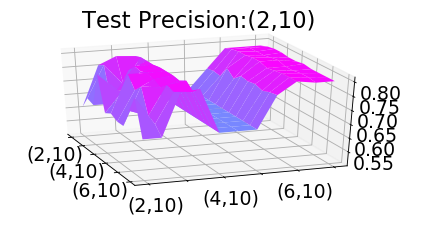
\includegraphics[width=0.5\textwidth]{210}
	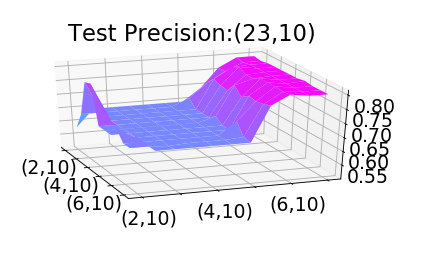
\includegraphics[width=0.5\textwidth]{2310}
	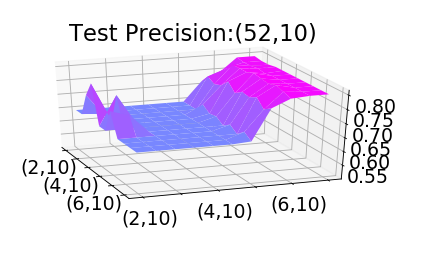
\includegraphics[width=0.5\textwidth]{5210}
\end{figure}

Provide just link to big datasets. 
Discussion sub section of Results.
\subsection{Discussion}

%% Acknowledgments
%\begin{acks}                            %% acks environment is optional
%                                        %% contents suppressed with 'anonymous'
%  %% Commands \grantsponsor{<sponsorID>}{<name>}{<url>} and
%  %% \grantnum[<url>]{<sponsorID>}{<number>} should be used to
%  %% acknowledge financial support and will be used by metadata
%  %% extraction tools.
%  This material is based upon work supported by the
%  \grantsponsor{GS100000001}{National Science
%    Foundation}{http://dx.doi.org/10.13039/100000001} under Grant
%  No.~\grantnum{GS100000001}{nnnnnnn} and Grant
%  No.~\grantnum{GS100000001}{mmmmmmm}.  Any opinions, findings, and
%  conclusions or recommendations expressed in this material are those
%  of the author and do not necessarily reflect the views of the
%  National Science Foundation.
%\end{acks}


%% Bibliography
\bibliography{bibfile}


%% Appendix
\appendix
\section{Appendix}

Text of appendix \ldots

\end{document}
